\section{Input images}
We consider 4 input images of different sizes.
\begin{figure}[h!]
\centering
\begin{subfigure}{0.5\textwidth}
  \centering
  
\includegraphics[width=0.5\linewidth]{../input/p0-1-0.jpg}
  \caption{Input p0-1-0.jpg, 207x236 pixels}
  \label{fig:sfig1}
\end{subfigure}%
\begin{subfigure}{0.5\textwidth}
  \centering
  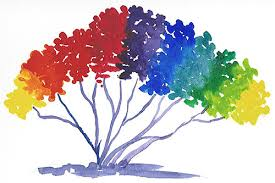
\includegraphics[width=0.5\linewidth]{../input/p0-1-1.jpg}
  \caption{Input p0-1-1.jpg, 183x275 pixels}
  \label{fig:sfig2}
\end{subfigure}
\begin{subfigure}{0.5\textwidth}
  \centering
  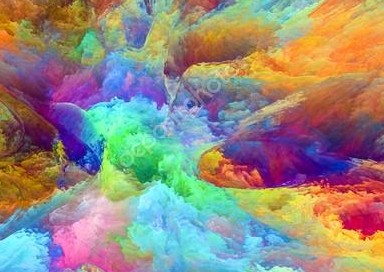
\includegraphics[width=0.5\linewidth]{../input/p0-1-2.jpg}
  \caption{Input p0-1-2.jpg, 272x384 pixels}
  \label{fig:sfig1}
\end{subfigure}%
\begin{subfigure}{0.5\textwidth}
  \centering
  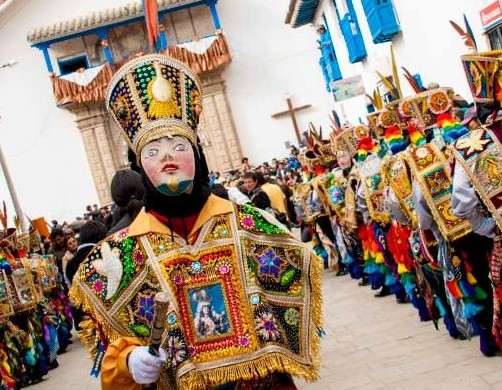
\includegraphics[width=0.5\linewidth]{../input/p0-1-3.jpg}
  \caption{Input p0-1-3.jpg, 390x502 pixels}
  \label{fig:sfig2}
\end{subfigure}
 \caption{Input images}
\label{fig:fig}
\end{figure}
